% Trial architecture diagram of LTCC following the user's master prompt (sans-serif, pastel regions A-F).
% Stand-alone; does not touch the manuscript. Build: pdflatex ltcc_arch.tex
\documentclass[tikz,border=3pt]{standalone}
\usepackage[T1]{fontenc}
\usepackage{tgheros}
\renewcommand{\familydefault}{\sfdefault}
\usepackage{sansmath}
\usepackage{amsmath,amssymb}
\usetikzlibrary{arrows.meta,calc,positioning}
% palette
\definecolor{ink}{HTML}{1C2733}
\definecolor{line}{HTML}{2B3A55}
\definecolor{cBlue}{HTML}{DCEBFA}   \definecolor{cBlueH}{HTML}{B9D6F2}
\definecolor{cCyan}{HTML}{D6F3F4}   \definecolor{cCyanH}{HTML}{A8E3E6}
\definecolor{cPeach}{HTML}{FDE6D6}  \definecolor{cPeachH}{HTML}{F8C9A8}
\definecolor{cLav}{HTML}{ECE6F7}    \definecolor{cLavH}{HTML}{D3C6EE}
\definecolor{cMint}{HTML}{DFF2E3}   \definecolor{cMintH}{HTML}{B5E0BE}
\definecolor{calib}{HTML}{C0392B}
\definecolor{fb}{HTML}{2F6DB5}
\definecolor{ground}{HTML}{F2F3F1}
\tikzset{
  every node/.style={text=ink},
  T/.style={font=\fontsize{7}{8.4}\selectfont\sansmath, align=center},
  Ts/.style={font=\fontsize{6.4}{7.7}\selectfont\sansmath, align=center},
  Tx/.style={font=\fontsize{5.9}{7}\selectfont\sansmath, align=center},
  Hd/.style={font=\fontsize{7.4}{8.8}\selectfont\sansmath, text=line},
  box/.style={draw=line, line width=0.55pt, rounded corners=2.5pt, align=center, inner sep=2.6pt},
  arr/.style={-{Stealth[length=4.4pt,width=3.5pt]}, line width=0.75pt, draw=ink},
  carr/.style={-{Stealth[length=3.8pt,width=3pt]}, line width=0.55pt, draw=calib},
  farr/.style={-{Stealth[length=4.2pt,width=3.4pt]}, line width=0.7pt, draw=fb, dash pattern=on 3pt off 1.8pt},
}
% \region{x1}{y1}{x2}{y2}{fill}{header fill}{title}
\newcommand{\region}[7]{%
  \filldraw[draw=line!70, line width=0.6pt, rounded corners=4pt, fill=#5!45] (#1,#2) rectangle (#3,#4);
  \fill[#6, rounded corners=4pt] (#1,{#4-0.45}) rectangle (#3,#4);
  \fill[#6] (#1,{#4-0.45}) rectangle (#3,{#4-0.25});
  \draw[line!70, line width=0.6pt, rounded corners=4pt] (#1,#2) rectangle (#3,#4);
  \node[Hd, anchor=west] at ({#1+0.12},{#4-0.225}) {#7};
}
% isometric slab: x, y, w, h, d, colour, text
\newcommand{\slab}[7]{%
  \filldraw[draw=line, line width=0.4pt, fill=#6!70!white] ({#1},{#2+#4}) -- ++({0.5*#5},{0.38*#5}) -- ++({#3},0) -- ++({-0.5*#5},{-0.38*#5}) -- cycle;
  \filldraw[draw=line, line width=0.4pt, fill=#6!60!black!35] ({#1+#3},{#2}) -- ++({0.5*#5},{0.38*#5}) -- ++(0,{#4}) -- ++({-0.5*#5},{-0.38*#5}) -- cycle;
  \filldraw[draw=line, line width=0.4pt, fill=white] ({#1},{#2}) rectangle ++({#3},{#4});
  \node[Ts] at ({#1+#3/2},{#2+#4/2}) {#7};
}
\newcommand{\badge}[2]{\node[font=\fontsize{5.6}{6}\selectfont, text=white, fill=#2, rounded corners=1.5pt,
  inner sep=1.5pt, anchor=east] at #1 {PROPOSED};}
\tikzset{
  quad/.pic={
    \foreach \dx/\dy in {-0.3/-0.09, 0.3/0.09, -0.11/0.15, 0.11/-0.15} \draw[line width=1pt, black!70] (0,0) -- (\dx,\dy);
    \foreach \dx/\dy in {-0.3/-0.09, 0.3/0.09, -0.11/0.15, 0.11/-0.15}
      \filldraw[draw=black!55, line width=0.3pt, fill=black!8] (\dx,\dy+0.04) ellipse (0.15 and 0.05);
    \filldraw[draw=black!80, line width=0.4pt, fill=#1] (0,0) ellipse (0.12 and 0.065);
  },
}
\begin{document}
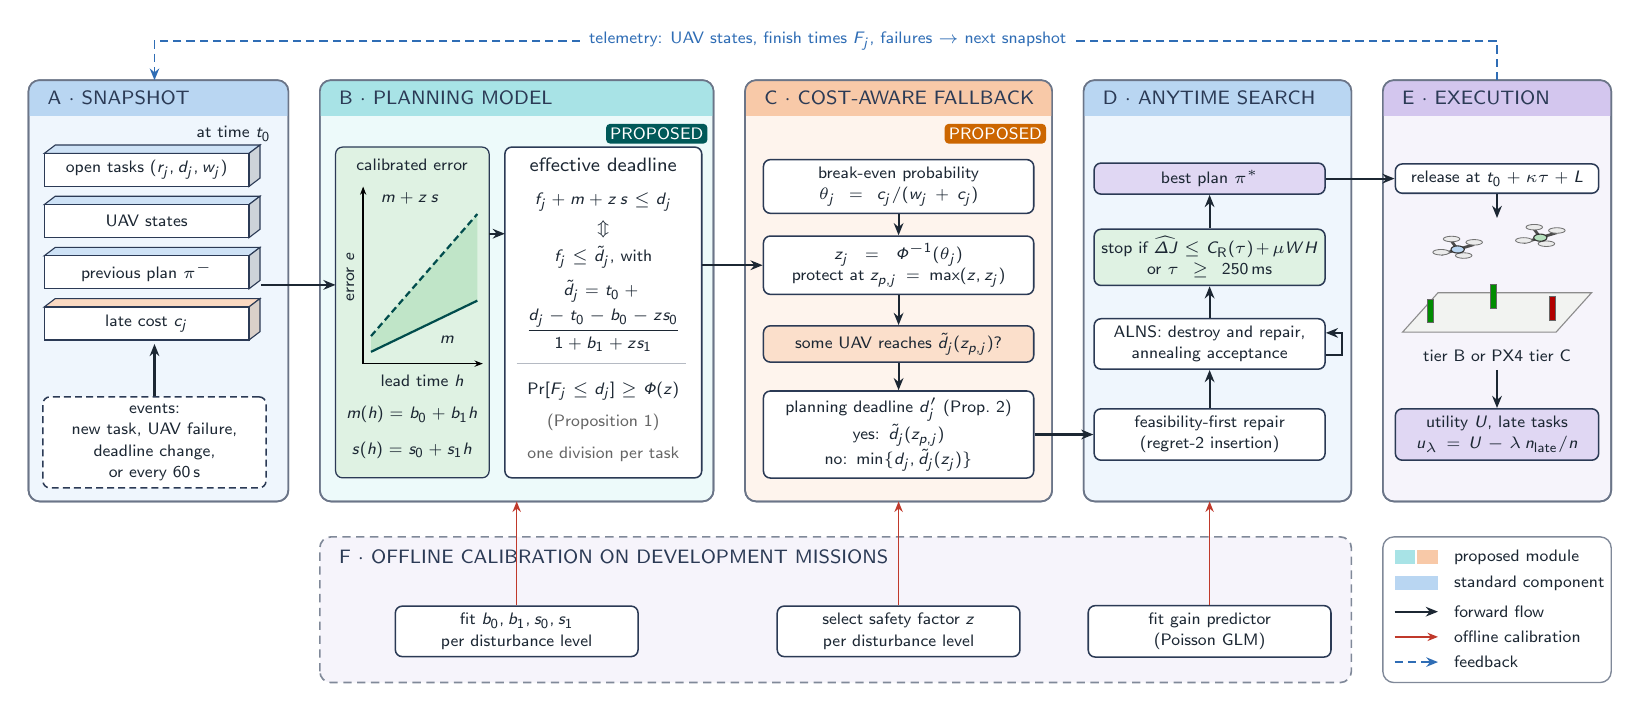
\begin{tikzpicture}

% ================================================================= regions
\region{0.15}{2.45}{3.45}{7.8}{cBlue}{cBlueH}{A $\cdot$ SNAPSHOT}
\region{3.85}{2.45}{8.85}{7.8}{cCyan}{cCyanH}{B $\cdot$ PLANNING MODEL}
\region{9.25}{2.45}{13.15}{7.8}{cPeach}{cPeachH}{C $\cdot$ COST-AWARE FALLBACK}
\region{13.55}{2.45}{16.95}{7.8}{cBlue}{cBlueH}{D $\cdot$ ANYTIME SEARCH}
\region{17.35}{2.45}{20.25}{7.8}{cLav}{cLavH}{E $\cdot$ EXECUTION}
\badge{(8.78,7.12)}{teal!70!black}
\badge{(13.08,7.12)}{orange!80!black}
% offline calibration group (dashed lavender)
\filldraw[draw=line!60, dash pattern=on 3pt off 2pt, line width=0.6pt, rounded corners=4pt, fill=cLav!45]
  (3.85,0.15) rectangle (16.95,2.0);
\node[Hd, anchor=west] at (3.97,1.75) {F $\cdot$ OFFLINE CALIBRATION ON DEVELOPMENT MISSIONS};

% ================================================================= A: snapshot
\slab{0.35}{6.45}{2.6}{0.42}{0.28}{cBlueH}{open tasks $(r_j,d_j,w_j)$}
\slab{0.35}{5.8}{2.6}{0.42}{0.28}{cBlueH}{UAV states}
\slab{0.35}{5.15}{2.6}{0.42}{0.28}{cBlueH}{previous plan $\pi^{-}$}
\slab{0.35}{4.5}{2.6}{0.42}{0.28}{cPeachH}{late cost $c_j$}
\node[box, dash pattern=on 2.5pt off 1.5pt, fill=white, text width=2.65cm, Ts] (ev) at (1.75,3.2)
  {events:\\ new task, UAV failure,\\ deadline change,\\ or every 60\,s};
\draw[arr] (ev.north) -- (1.75,4.45);
\node[Ts, anchor=east] at (3.35,7.12) {at time $t_0$};

% ================================================================= B: error model and effective deadline
\filldraw[draw=line, line width=0.45pt, rounded corners=2.5pt, fill=cMint] (4.05,2.75) rectangle (6.0,6.95);
\node[Ts] at (5.02,6.72) {calibrated error};
\fill[cMintH!85] (4.5,4.55) -- (5.85,6.1) -- (5.85,5.0) -- (4.5,4.35) -- cycle;
\draw[line width=0.8pt, teal!60!black] (4.5,4.35) -- (5.85,5.0);
\draw[line width=0.8pt, teal!60!black, dash pattern=on 2.4pt off 1.4pt] (4.5,4.55) -- (5.85,6.1);
\draw[-{Stealth[length=3pt]}, line width=0.5pt] (4.4,4.2) -- (5.92,4.2);
\draw[-{Stealth[length=3pt]}, line width=0.5pt] (4.4,4.2) -- (4.4,6.45);
\node[Tx, anchor=north] at (5.15,4.18) {lead time $h$};
\node[Tx, rotate=90] at (4.24,5.3) {error $e$};
\node[Tx, anchor=west] at (4.5,6.3) {$m+z\,s$};
\node[Tx, anchor=west] at (5.25,4.5) {$m$};
\node[Ts] at (5.02,3.55) {$m(h)=b_0+b_1h$};
\node[Ts] at (5.02,3.1) {$s(h)=s_0+s_1h$};
% effective deadline (novel)
\filldraw[draw=line, line width=0.55pt, rounded corners=2.5pt, fill=white] (6.2,2.75) rectangle (8.7,6.95);
\node[T] at (7.45,6.72) {effective deadline};
\node[Ts] at (7.45,6.25) {$f_j+m+z\,s\le d_j$};
\node[Ts] at (7.45,5.9) {$\Updownarrow$};
\node[Ts] at (7.45,5.55) {$f_j\le\tilde d_j$, with};
\node[Ts] at (7.45,5.12) {$\tilde d_j=t_0+{}$};
\node[Tx] at (7.45,4.62) {$\dfrac{d_j-t_0-b_0-z s_0}{1+b_1+z s_1}$};
\draw[line!35, line width=0.4pt] (6.35,4.2) -- (8.5,4.2);
\node[Ts] at (7.45,3.85) {$\Pr[F_j\le d_j]\ge\Phi(z)$};
\node[Tx, text=black!60] at (7.45,3.45) {(Proposition 1)};
\node[Tx, text=black!60] at (7.45,3.05) {one division per task};
\draw[arr] (6.0,5.85) -- (6.2,5.85);

% ================================================================= C: cost-aware fallback
\node[box, fill=white, text width=3.25cm, Ts] (c1) at (11.2,6.45) {break-even probability\\ $\theta_j=c_j/(w_j+c_j)$};
\node[box, fill=white, text width=3.25cm, Ts] (c2) at (11.2,5.45) {$z_j=\Phi^{-1}(\theta_j)$\\ protect at $z_{p,j}=\max(z,z_j)$};
\node[box, fill=cPeachH!60, text width=3.25cm, Ts] (c3) at (11.2,4.45) {some UAV reaches $\tilde d_j(z_{p,j})$?};
\node[box, fill=white, text width=3.25cm, Ts] (c4) at (11.2,3.3) {planning deadline $d'_j$ (Prop.~2)\\
  yes: $\tilde d_j(z_{p,j})$\\ no: $\min\{d_j,\tilde d_j(z_j)\}$};
\draw[arr] (c1) -- (c2);
\draw[arr] (c2) -- (c3);
\draw[arr] (c3) -- (c4);

% ================================================================= D: anytime search (standard components)
\node[box, fill=white, text width=2.75cm, Ts] (d1) at (15.15,3.3) {feasibility-first repair\\ (regret-2 insertion)};
\node[box, fill=white, text width=2.75cm, Ts] (d2) at (15.15,4.45) {ALNS: destroy and repair,\\ annealing acceptance};
\node[box, fill=cMint, text width=2.75cm, Ts] (d3) at (15.15,5.55) {stop if $\widehat{\Delta J}\le C_{\mathrm R}(\tau)+\mu W H$\\ or $\tau\ge 250$\,ms};
\node[box, fill=cLavH!70, text width=2.75cm, Ts] (d4) at (15.15,6.55) {best plan $\pi^\ast$};
\draw[arr] (d1) -- (d2);
\draw[arr] (d2) -- (d3);
\draw[arr] (d3) -- (d4);
\draw[arr] ([yshift=-4pt]d2.east) -- ++(0.2,0) |- ([yshift=4pt]d2.east);

% ================================================================= E: execution
\node[box, fill=white, text width=2.4cm, Ts] (e1) at (18.8,6.55) {release at $t_0+\kappa\tau+L$};
\filldraw[draw=black!45, line width=0.4pt, fill=ground] (17.6,4.6) -- (19.55,4.6) -- (20.0,5.1) -- (18.05,5.1) -- cycle;
\foreach \x/\y/\c in {17.95/4.72/green!55!black, 18.75/4.9/green!55!black, 19.5/4.75/red!70!black}
  \filldraw[draw=black!60, line width=0.3pt, fill=\c] (\x-0.04,\y) rectangle ++(0.08,0.3);
\pic[scale=0.7] at (18.3,5.65) {quad=cBlueH};
\pic[scale=0.7] at (19.35,5.8) {quad=cMintH};
\node[Ts] at (18.8,4.3) {tier B or PX4 tier C};
\node[box, fill=cLavH!70, text width=2.4cm, Ts] (e3) at (18.8,3.3) {utility $U$, late tasks\\ $u_\lambda=U-\lambda\,n_{\mathrm{late}}/n$};
\draw[arr] (e1.south) -- (18.8,6.05);
\draw[arr] (18.8,4.12) -- (e3.north);

% ================================================================= main forward flow between regions
\draw[arr] (3.1,5.2) -- (4.05,5.2);
\draw[arr] (8.7,5.45) -- (c2.west);
\draw[arr] (c4.east) -- (d1.west);
\draw[arr] (d4.east) -- (e1.west);

% ================================================================= feedback (dashed blue)
\draw[farr] (18.8,7.8) -- (18.8,8.3) -- (1.75,8.3) -- (1.75,7.8);
\node[Ts, fill=white, inner sep=1.5pt, text=fb] at (10.3,8.3) {telemetry: UAV states, finish times $F_j$, failures $\rightarrow$ next snapshot};

% ================================================================= F: offline calibration (thin red)
\node[box, fill=white, text width=2.9cm, Ts] (f1) at (6.35,0.8) {fit $b_0,b_1,s_0,s_1$\\ per disturbance level};
\node[box, fill=white, text width=2.9cm, Ts] (f2) at (11.2,0.8) {select safety factor $z$\\ per disturbance level};
\node[box, fill=white, text width=2.9cm, Ts] (f3) at (15.15,0.8) {fit gain predictor\\ (Poisson GLM)};
\draw[carr] (f1.north) -- (6.35,2.45);
\draw[carr] (f2.north) -- (11.2,2.45);
\draw[carr] (f3.north) -- (15.15,2.45);

% ================================================================= legend
\begin{scope}[shift={(17.35,0.15)}]
\filldraw[draw=line!60, line width=0.5pt, rounded corners=4pt, fill=white] (0,0) rectangle (2.9,1.85);
\fill[cCyanH] (0.15,1.5) rectangle ++(0.26,0.18); \fill[cPeachH] (0.44,1.5) rectangle ++(0.26,0.18);
\node[Tx, anchor=west] at (0.78,1.59) {proposed module};
\fill[cBlueH] (0.15,1.17) rectangle ++(0.55,0.18);
\node[Tx, anchor=west] at (0.78,1.26) {standard component};
\draw[arr] (0.15,0.9) -- ++(0.55,0); \node[Tx, anchor=west] at (0.78,0.9) {forward flow};
\draw[carr] (0.15,0.58) -- ++(0.55,0); \node[Tx, anchor=west] at (0.78,0.58) {offline calibration};
\draw[farr] (0.15,0.26) -- ++(0.55,0); \node[Tx, anchor=west] at (0.78,0.26) {feedback};
\end{scope}
\end{tikzpicture}
\end{document}
